\chapter{Deep learning neural networks}
\label{chap:deep}
\section{Context}
Deep learning neural networks gained popularity again in recent years, after the AI winter ended. Since then neural networks became part of the everyday life, we hear about artificial intelligence being used in smart phones to enhance images quality or recognize certain settings and take a picture accordingly. AI is also being used in cancer research and other fields of bioinformatics, and personal assistants became extremely popular as well.

But even with the seemingly endless capabilities of artificial neural networks we are far from creating anything that could have the cognitive capacities of humans. This problem is considered by many to be AI-complete or AI-hard, meaning that creating a network that could keep up a human-like conversation would require data scientist and researchers to construct a universal artificial intelligence. A small but important step to achieve this is to create a system capable of doing simple reading comprehension tasks that also require some common sense knowledge.

The most common structures of these experimental neural networks include recurrent neural network layers and attention layers. Before we explain the function of these building-blocks we need to lay down a foundation.

In this chapter we will introduce the deep learning mechanisms that are the essential building blocks of the Yuanfudao system described in Chapter \ref{chap:yuanfudao}.

\section{Basics}
\begin{minipage}{\textwidth}
Some arbitrary definitions we will use in this chapter:
\begin{itemize}
	\item \textbf{Batch}: The chunks of training data that we use for training in one iteration. It's size can be a crucial parameter to set.
	\item \textbf{Epoch}: One training iteration is called an epoch. The number of epochs determines how long we want to train our network.
	\item \textbf{Learning rate}: \(\eta\) the velocity of the learning process. Setting it too low could result in slow learning and getting stuck in a local minimum, but setting it too high could result in jumping over the optimum and bouncing.
	\item \textbf{Accuracy}: The ratio of the correct predictions and the all prediction. Our goal is to achieve a high accuracy with our neural network on the test set.
	\item \textbf{Test set}: The part of the dataset that we don't use during the training of our neural network. This determines the actual accuracy of the network.
	\item \textbf{Training set}: The data we could use for training our network is usually split into two parts in 80:20 ratio. We use the bigger set of data to train our network and we call this the training set.
	\item \textbf{Development set or Validation set}: The smaller portion of the data. We use this section to validate the network during its training. We do not use this section of the data to train the network.
\end{itemize}
\end{minipage}
\\
\\
People usually use supervised learning in the field of natural language processing to achieve the desired structure, but we might face multiple challenges while training. That's reason why we have to use optimization and regularization methods.

\subsection{Optimization}
The goal of optimization is to overcome the following problems:
\begin{itemize}
	\item Local minimum
	\item Setting the learning rate
	\item Setting the batch size
\end{itemize}

We have touched on the first two briefly before, but setting the batch size is also very important. We give the training data to the network in batch-es, and we iterate through them multiple times (depending on the epoch). The loops length is the number of epochs we take.

Methods used for optimizing:
\begin{itemize}
	\item \textbf{Stochastic gradient descent}
	\item \textbf{Momentum}
	\item \textbf{Adaptive learning rate}
	\item \textbf{Adam} (Adaptive learning rate and momentum)
	\item \textbf{AdaMax} (Adam variant)
\end{itemize}

\paragraph*{Stochastic gradient descent}
\[g \leftarrow \frac{1}{batchSize}\Delta_w \sum_{i=1}^{batchSize}Loss(f_w(x_i), y_i)\]
Where f is the network itself.
\[w \leftarrow w - \eta g\]
This is a classical method for optimizing. It does not account for dynamic parameter settings. The system described in Chapter \ref{chap:yuanfudao} can use this function.
We will consider this as our base, and only highlight the differences between this and other optimization methods.

\paragraph*{Momentum}
\[g \leftarrow \alpha g + \frac{1}{batchSize}\Delta_w \sum_{i=1}^{batchSize}Loss(f_w(x_i), y_i)\]
Where \(\alpha\) is a parameter we can set.
This method has an added parameter, that helps to take into account the previous iterations, giving a momentum to the learning towards the optimum.

\paragraph*{Adaptive learning rate}
\[r \leftarrow r + g^2\]
Where r is a parameter thats initial value can be set.
\[w \leftarrow w - \frac{\eta}{\sqrt{r}} g\]
As the name suggests the adaptive learning rate uses a parametrization to slowly decrease the learning rate through time, depending on the previously calculated gradient.

\paragraph*{Adam}
\[r \leftarrow \varphi_r r + (1 - \varphi_r) g^2\]
\[s \leftarrow \varphi_s s + (1 - \varphi_s) g\]
Where s is a parameter thats initial value can be set and \(\varphi\) is a parameter of the decay rate.
\[w \leftarrow w - \frac{\eta s}{\sqrt{r}} g\]
Adam is one of the most popular optimizer function nowadays. It combines the adaptive learning rate and the momentum hence the name: Adam.

\paragraph*{AdaMax}
\[r \leftarrow \max(\varphi_r r, |g|)\]
\[s \leftarrow \varphi_s s + (1 - \varphi_s) g\]
\[w \leftarrow w - \frac{\eta}{1 - \varphi_s}\frac{s}{r}\]
A variant of the Adam optimizer. It was first described in the \textit{Adam: A method for stochastic optimization} article \cite{Kingma:2015}. It differs from Adam in that it uses a max operation and the infinity norm. The system described in Chapter \ref{chap:yuanfudao} can use this optimization function too.

\subsection{Regularization}
The goal of regularization is to avoid over-fitting. Over-fitting happens when our neural network produces good results on the training set's dedicated subset, the development or validation set, but it can't predict the expected outputs properly on a new dataset for example the test set. It happens very often, so machine learning experts developed a couple functions to avoid this phenomenon.
\begin{itemize}
	\item \textbf{Weight decay}: Also known as L2 regularization. It uses a parameter to make sure that the previously learned weight won't influence the new one too much. \[w \leftarrow (1 - \eta \alpha)w - \eta \Delta_w Loss\]
	\item \textbf{L1 regularization}: This is a normalization method that modifies the cost function similarly to the L2 regularization. The difference is, that in this case the weights might get reduced to zero.
	\item \textbf{Dropout}: It randomly disables weights for an epoch, so they won't used in that iteration
	\item \textbf{Early stopping}: It stops the learning if the results on the development set haven't shown any progress in the last couple of epochs.
	\item \textbf{Noise injection}: It injects noise into the training set.
\end{itemize}

The system later described in Chapter \ref{chap:yuanfudao} uses dropouts while learning. This might cause the system's performance to fluctuate a little bit from epoch to epoch but it is a powerful tool for regularization and as we'll see later it manages to achieve consistently good results on the development set.

\section{Natural Language Processing with Deep learning}
As mentioned above the kind of layers used in Natural Language Processing are mostly recurrent neural network layers, attention layers and sometimes embedding layers.

\subsection{Embedding layers}

The function of embedding layers is to turn integer values to fixed length vectors, for example word embedding vectors discussed in Chapter \ref{chap:semanticparsing}. They are used mostly in natural language processing to work as word2vec translation.

When using embedding layers we want to find vectors for each word so that it can model the word's meaning. We achieve this by looking at the context, the word usually appears in. If two words like \textit{apple} and \textit{orange} usually appear in the same context, than the vectors assigned to these words should have low cosine distance between them. You can read about this idea in detail in Chapter \ref{chap:semanticparsing}.

If you are building an NLP model, the embedding layer should be in the first layer, since its purpose is to make the transition from word to vector, and the word in this case is the input.

\begin{figure*}[!htb]
	\centering
	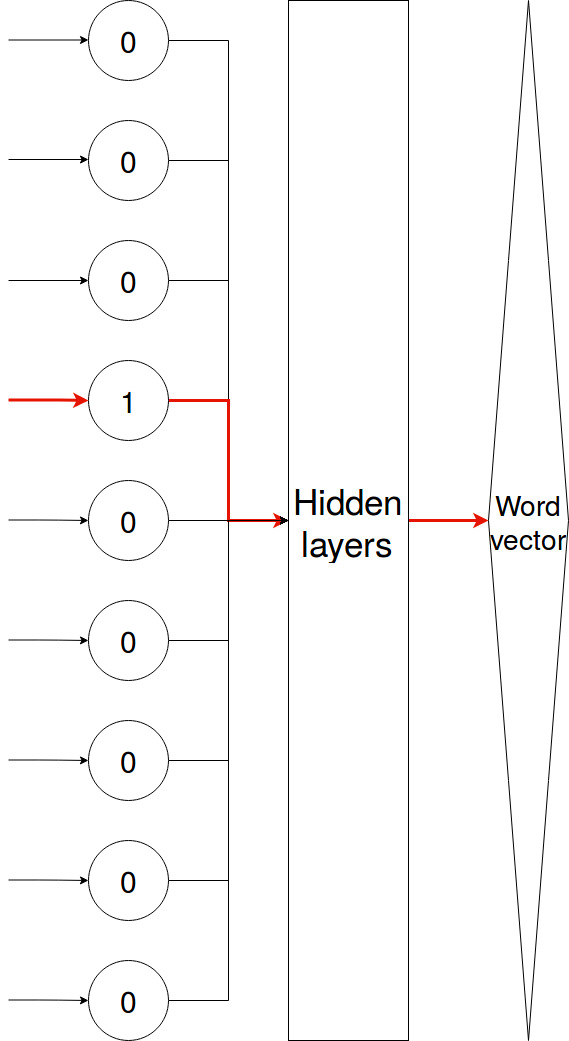
\includegraphics[scale=0.25]{embedding_layer.jpg}
	\caption{An embedding layer.}
	\label{fig:embedding_layer}
\end{figure*}

The input dimension of this layer is the size of the vocabulary and the output dimension is the size of the dense vector. Usually the vocabulary size greatly exceeds the embedding dimension since the output vectors size is fixed and can range from 300 to 1000, and the vocabulary - depending on the dataset - can be way higher than that. See at Figure~\ref{fig:embedding_layer}.

They work mostly like a lookup table that can be trained. A lot of the times we use pretrained models, like the GloVe embeddings that have been trained on enormous datasets. We can also train them on our specific problem, or use the pretrained and our own embeddings simultaneously.
\FloatBarrier

\subsection{Recurrent Neural Networks}

In a simple feed forward neural network, the information only moves in one direction: from the input layer to the output layer. On the other hand recurrent neural networks take into account their immediate past, the output of the network with the previous timestamp. This internal "memory" like functionality allows the network to remember what it had calculated before. This is illustrated at Figure~\ref{fig:recurrent_net}.

At every timestamp the network gets two set of inputs: the actual input at the timestamp and the hidden state of the network for the previous input. In one iteration it calculates its output using the calculated hidden state in the timestamp. It all could be imagined like the same feed forward network being repeated after one other.

The hidden state mentioned above is the "memory" of the network that is calculated with the previous hidden state and the input.

\begin{figure*}[!htb]
	\centering
	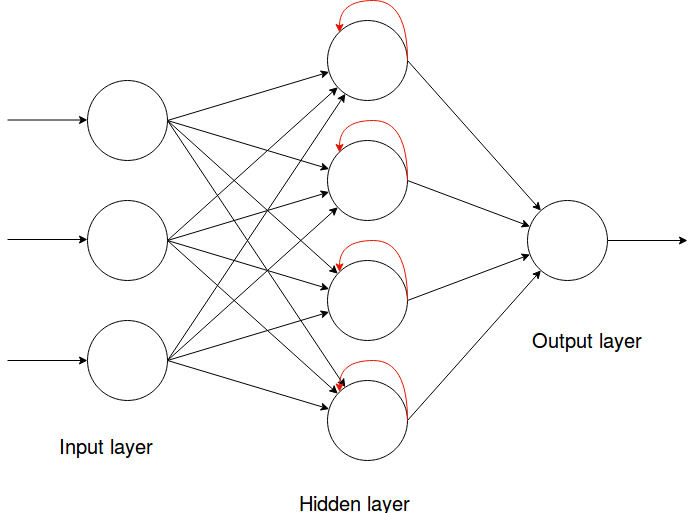
\includegraphics[scale=0.5]{recurrent_neural_network.jpg}
	\caption{A recurrent neural network.}
	\label{fig:recurrent_net}
\end{figure*}

The backpropagation is also slightly different in this case, it's called backpropagation through time, you need to "unroll" the network (see at Figure~\ref{fig:unrolled}), and use the backpropagation starting from the right timestamps. Each timestamp's backpropagation could be understood as backpropagation on a separate feed forward neural network. 
\begin{figure*}[!htb]
	\centering
	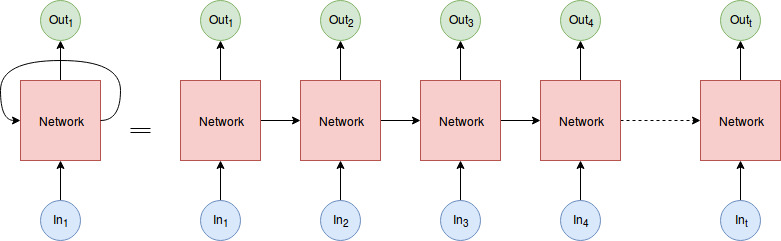
\includegraphics[scale=0.5]{unrolled.jpg}
	\caption{Unrolled recurrent neural network.}
	\label{fig:unrolled}
\end{figure*}

The gradient vanishing or explosion can be a problem with this RNN.

There is a multitude of solutions for the exploding gradients, one of which is called gradient clipping. This is one of the method the state-of-the art system, Yuanfudao uses.

This technique is a very simple yet powerful way of dealing with exploding gradients. All it does is that it limits the size of the gradient, if it norm is higher than a set threshold.

RNNs can be used in supervised and also unsupervised learning. They are used when the data is sequential, like text, audio, etc.

\subsubsection{Long-Short Term Memory}
The system we worked with uses LSTM layers as its default RNN type.
Long-short term memory networks ar the extension of the previously discussed recurrent neural network. The main difference is that it also has an internal long term memory. Usually these type of networks are more reluctant to have the exploding gradient problem.

Like the simple RNN, LSTMs also have hidden states, that are calculated slightly differently.
\\

\begin{minipage}{\textwidth}
The LSTMs hidden states are calculated using three gates:
\begin{itemize}
	\item \textbf{input gate}: determines whether to let new input in
	\item \textbf{forget gate}: determines whether to forget an input because it's not relevant anymore
	\item \textbf{output gate}: determines whether to let the input impact the output with the current timestamp
\end{itemize}
\end{minipage}

These gates are analog and their value ranges from 0 to 1 with the sigmoid function. A simplified depiction can be seen at Figure~\ref{fig:lstm}\footnote{\url{https://en.wikipedia.org/wiki/Long_short-term_memory}}.
\begin{figure*}[!htb]
	\centering
	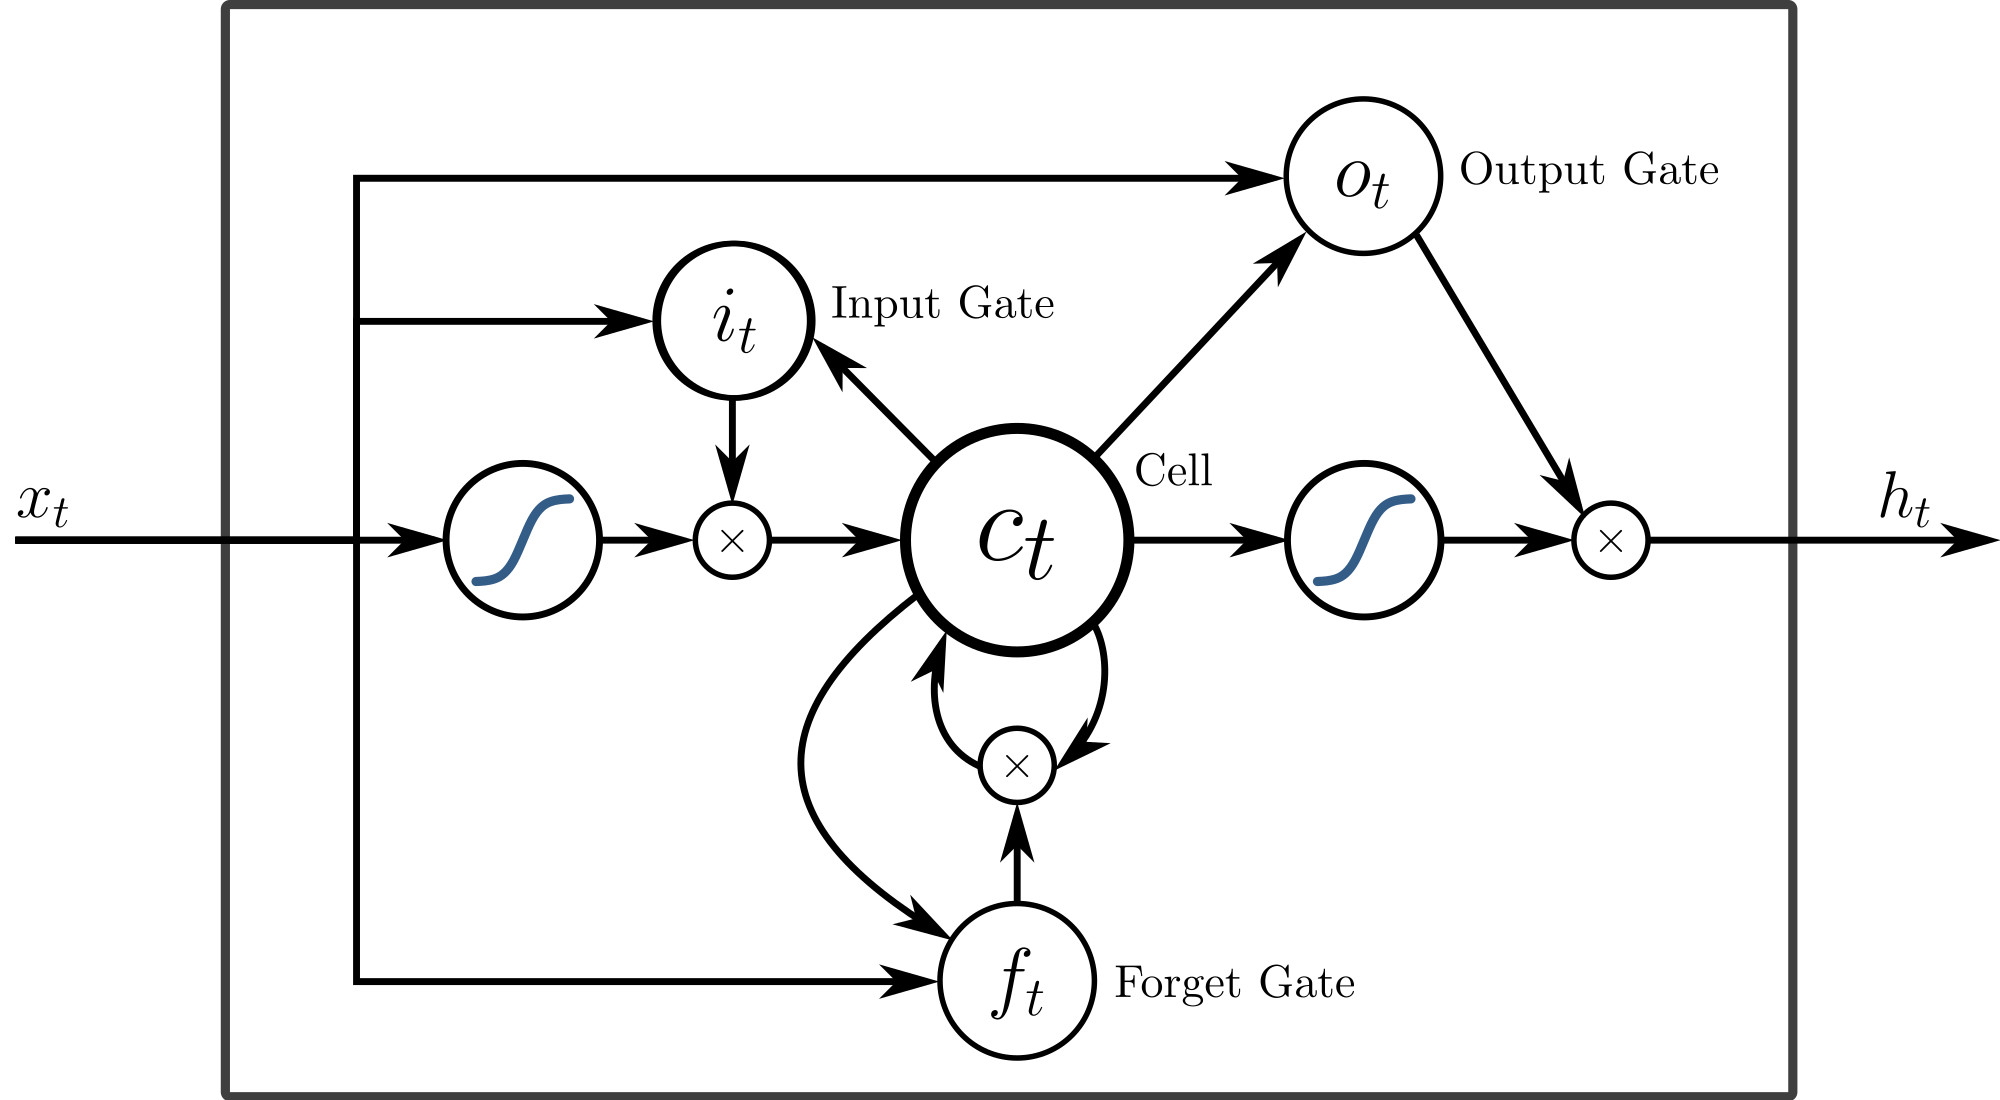
\includegraphics[scale=0.2]{lstm.jpg}
	\caption{A long-short term memory network's gates.\\Image from Wikipedia}
	\label{fig:lstm}
\end{figure*}
\FloatBarrier

The sigmoid function allows this structure to be able to learn, meaning that we can use the backpropagation through time method described above.

Long-short term memory networks are used in natural language processing, but also in generative networks, like video or image description generation, text generation and so on.

\paragraph*{Bidirectional long-short term memory} also known as BiLSTM\\
BiLSTM networks are a variant of long-short term memory that read the input from the beginning to the end than also from the end to the beginning. The main idea behind this is that we may need not just the previous output, but also the next one too. These networks usually outperform simple LSTM systems in their predictions and the learning velocity too.

\subsubsection{Gated recurrent unit}
The system we worked with can use GRU layers as its RNN type, but it's not its default setting and it did not perform as good.
Gated recurrent units are also a type of RNN and have a similar structure (Figure~\ref{fig:gru}\footnote{\url{https://en.wikipedia.org/wiki/Gated_recurrent_unit}}) to the long-short term memory network, but has been shown to exhibit better performance on smaller datasets, than the LSTM.
\begin{figure*}[!htb]
	\centering
	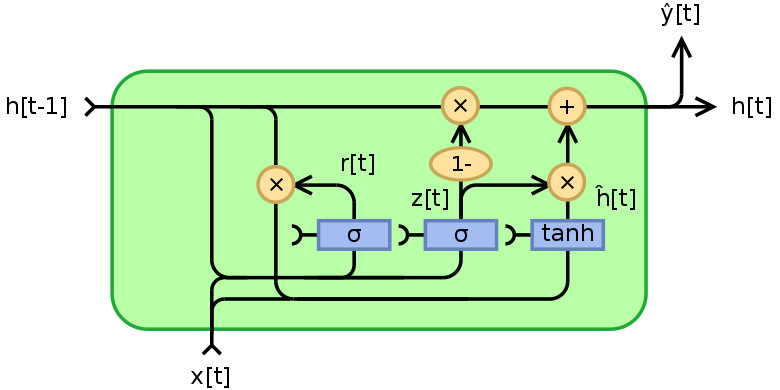
\includegraphics[scale=0.5]{gru.jpg}
	\caption{A gated recurrent unit's gates.\\Image from Wikipedia}
	\label{fig:gru}
\end{figure*}

\begin{minipage}{\textwidth}
It has four main building blocks:
\begin{itemize}
	\item \textbf{update gate}: the gate gets the x[t] and the h[t-1] as its input and z[t] is the output on the image
	\item \textbf{reset gate}: the gate gets the x[t] and the h[t-1] as its input and r[t] is the output on the image
	\item \textbf{current memory content}: the gate gets the x[t], the h[t-1] and the r[t] as its input and \^{h}[t] is the output on the image
	\item \textbf{final memory at current time step}: the h[t] on the image
\end{itemize}
\end{minipage}

Gated recurrent units are mostly used on the field of speech recognition and music modeling while the LSTM is more relevant on the field of natural language processing.

\subsection{Attention}
The Attention mechanism was first described in \cite{Bahdanau:2015} and was used for machine translation. Since then it became a widely used tool in natural language processing. The idea behind this mechanism is that when the neural network predicts the output, it only uses parts of the given input instead of the full input. That is where the most relevant informations are concentrated and this mechanism only pays \textit{attention} to these parts and the network has to learn what to pay attention to.

Usually in the "sequence-to-sequence" tasks like MT there are two main parts of the model an encoder and a decoder. The encoder and the decoder are usually some type of RNN, mostly LSTM. The encoder is responsible for creating a so called context-vector from the input sequence. This context-vector has a fixed length and it serves as the representation of the sequence inside the model. The decoder then decodes this context-vector to a sequence again, in the case of the machine translation this sequence is in a different language. A depiction can be seen at Figure~\ref{fig:seq_to_seq}.
\begin{figure*}[!htb]
	\centering
	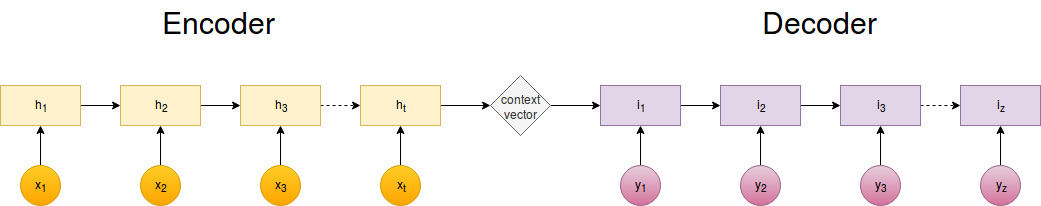
\includegraphics[scale=0.4]{seq_to_seq.jpg}
	\caption{A sequence-to-sequence model with encoder and decoder.}
	\label{fig:seq_to_seq}
\end{figure*}

The attention mechanism described in \cite{Bahdanau:2015} was used in the decoder part of this model, the encoder functions the same way. The paper explicitly stated that this attention mechanism relieves the encoder from having to encode every sequence to a fixed length context vector. In this case we have a context vector for every word of the expected output. These context-vectors are the weighted sums of the encoder's states (\textit{annotations}).
\[c_i = \sum_{j=1}^{t} \alpha_ij h_j\]
Where \(\alpha\) parameter is calculated like the following:
\[\alpha_ij = \frac{exp(e_{ij})}{\sum_{k=1}^{t} e_{ik}} \]
and \(e_{ij}\) is its energy
\[e_{ij} = a(s_{i-i}, h_j)\]
This is an \textit{alignment model} that scores how well the input around \textit{j} and the output around \textit{i} match. This \textit{alignment model} is a feed forward neural network that is trained simultaneously with the other components of the system.
The decoder uses the previous state's output and its assigned context-vector when calculating its own target.
\[s_i = f(s_{i-1}, y_{i-1}, c_i)\]
The attention based model is at Figure~\ref{fig:attention}.
\begin{figure*}[!htb]
	\centering
	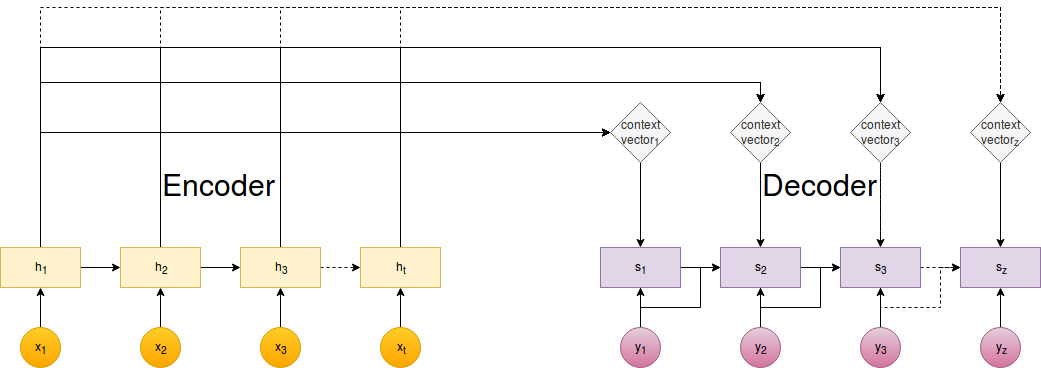
\includegraphics[scale=0.4]{attention.jpg}
	\caption{A sequence-to-sequence model with encoder-decoder and attention.}
	\label{fig:attention}
\end{figure*}

A big advantage of using this mechanism is the ability to interpret our model. These days it's more important than ever to be able to tell why does the network predict what it predicts, and thanks to the attention mechanism we are able to say that (in a purely attention-based network). One example is shown at Figure~\ref{fig:interpretation}.

\begin{figure*}[!htb]
	\centering
	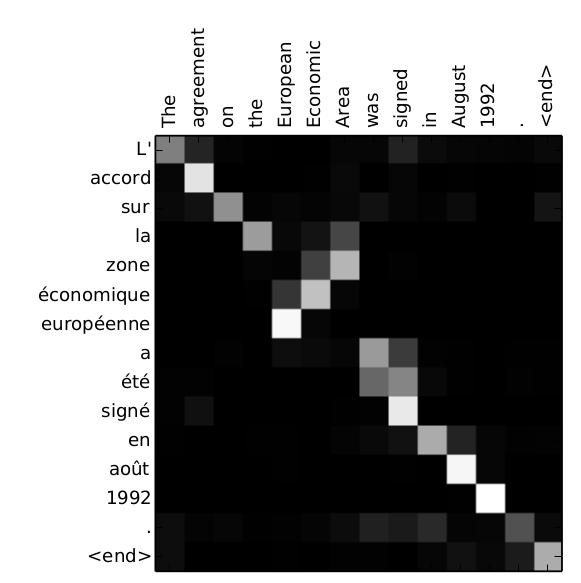
\includegraphics[scale=0.5]{interpretation.jpg}
	\caption{An interpretation of a french - english sequence to sequence translation.\\Image from \cite{Bahdanau:2015}.}
	\label{fig:interpretation}
\end{figure*}

\begin{minipage}{\linewidth}
	Since its first description in \cite{Bahdanau:2015} the attention mechanism has been used for:
	\begin{itemize}
		\item \textbf{Image caption/description}: a convolutional neural network translates the image to the context vectors and the decoder creates a description for it. A recent system using attentions for image captioning is described in the \textit{Image Caption with Global-Local Attention} paper \cite{Li:2017c}.
		\item \textbf{Grammar representation}: in this case the decoder builds a grammatical representation for the input. On a related field there was a study regarding linguistic representations and attentions \cite{Kadar:2016}.
		\item \textbf{Advanced machine translation}: Since it was first introduced it has revolutionized the field of machine translation. A study on this field is \textit{Effective Approaches to Attention-based Neural Machine Translation} \cite{Luong:2015b}.
		\item \textbf{Machine comprehension tasks}: question answering based on a previously read text. The system described in Chapter \ref{chap:yuanfudao} is like this \cite{Wang:2018}.
	\end{itemize}
\end{minipage}